\documentclass[12pt, twocolumn]{article}
\usepackage[margin=1in]{geometry}
\usepackage{amsmath,amssymb,amsthm}
\usepackage{graphicx}
\usepackage{hyperref}

\begin{document}
\title{LEGATO: Latent Embedding Gradient Aware Trajectory Optimization}
\date{May 17, 2024}
\maketitle
\begin{abstract}
    Gradient-enabled optimization methods are highly effective in robotic control problems.
    By enabling gradient-based methods to work in learned dynamics models, effective and stable control can be realized for environments which are too complex to model manually.
    This work investigates an approach that plans online using smooth learned representations of both states and actions.
    A smoothness constraint on the latent space simplifies planning by allowing gradient-based methods to be employed.
\end{abstract}
\section{Introduction}
Learning forward models and latent spaces are both topics which have been extensively investigated.
Existing approaches, however, generally focus on sampling based optimization methods in the planned spaces.
This is more feasible for learned state space models because sampling based optimizers generally are more effective in spaces that are unsmooth and non-convex.
In ground truth spaces there are generally multiple disconnected optimal solutions, and sudden discontinuities in the dynamics such those created by walls.
This makes them unsmooth and non-convex, and thus makes them unsuitable for gradient-based optimization.
Learned state spaces cannot be assumed to be smooth or convex when learned by general approximators like neural networks.
This work investigates the feasibility of constraining a learned representation and forward model to be smooth, as well as the effects that this constraint has on gradient-based optimization

\section{Related Work}

This problem is well-studied in the control and reinforcement learning literature.
Several other works have sought to achieve similar task-agnostic control.

In model based approaches several methods train approximators which enable control in dynamic systems \cite{williams_information_2017,chua_deep_2018,lambert_low_2019}.
These works learn a dynamics model and then plan using these learned dynamics models.
Existing approaches for online planning with Model Based Reinforcement Learning (MBRL) fall short in that they all use sampling based methods to find trajectories.
While these sampling based methods are effective for finding feasible control in relatively simple control environments, more complex scenarios require prohibitively many samples and result in very noisy convergence.

Another common approach to online planning for diverse goals comes from robotic foundation models.
These models aim to learn planning using a very powerful model and then generalize these capabilities at test time.
This approach shows a lot of success in works such as the robot transformer line of work \cite{brohan_rt-1_2022,brohan_rt-2_2023,padalkar_open_2023}.
Training such large models is very computationally expensive and they are too large to deploy on-board even for larger robots.
These issues make this approach infeasible for high-frequency control on most robotic systems.

A third approach that is used for diverse test-time control is Embed To Control \cite{watter_embed_2015} which applies a very strict constraint to a learned model of the system dynamics which is that it must be locally linear.
Such efforts are effective for continuous controllable systems but require the system can be approxoimated linearly.
For this reason such methods are mainly suited for recovering embeddings from high dimensional data in broadly controllable systems.

Learned world models have also been used both in learned latent spaces \cite{hafner_dream_2020} and ground truth spaces \cite{lowrey_plan_2019}.
Generally these approaches use a learned latent state space to extract low dimensional information rather than to enforce any convenient properties on the latent space.

\section{Approach}

Given a state space \(\mathcal{S}\) and action space \(\mathcal{A}\) of an \(M\!D\!P\setminus\!R\): \(\{\mathcal{S}, \mathcal{A}, \mathcal{P}\}\) a latent state and action space are learned that the transition dynamics within the latent space obey P-Lipchitz Continuity.
The latent spaces corresponding to the ground truth \(M\!D\!P\setminus\!R\) are \(\mathcal{Z}_s\) and \(\mathcal{Z}_a\).
The latent state and action encoders are \(E_s: \mathcal{S} \rightarrow \mathcal{Z_s}\) and \(E_a: \mathcal{A} \times \mathcal{S} \rightarrow \mathcal{Z_a}\) respectively.
The state is passed to the state encoder to allow latent action embeddings to vary by states.
For example stepping forward on a cliff represents a very different action than stepping forward on a sidewalk.
An additional function is learned which is the latent transition model \(T: \mathcal{Z_s} \times \mathcal{Z_a} \rightarrow \{Z_s\}\) which predicts the future state based on a state and an action.

To make this space amenable to gradient-based optimization the latent state and action spaces are constrained to be Lipschitz continuous within a small radius with respect to the transition model.
This constraint is expressed in the following inequality.
\[\|z_a - z_a'\|_p \leq \gamma^{-1} \|T(z_s, z_a) - T(z_s, z_a')\|_p\]

This is generalized to multiple steps as follows:
\[\|z_a - z_a'\|_p \leq \gamma^{-t} \|T(z_s, \mathbf{z}_{a, 0:t}) - T(z_s, \mathbf{z}_{a, 0:t}')\|_p\]

Where \(\mathbf{z}_{a, 0:t}\) is a sequence of actions up to time \(t\), \(z_a\) is the first action, \(z_a'\) is a perturbed version of the first action, and \(\mathbf{z}_{a,0:t}'\) is the same action sequence with \(z_a'\) at the start instead of \(z_a\).

To apply this constraint the loss \(\mathcal{L}_\text{smooth}\) is used.
\begin{multline*}
    \mathcal{L}_\text{smooth} = \\
    \underset{t<H,\;(z_s,\mathbf{z}_{a,0:H})\in E(D)}{E} \text{relu}\!\big[\|z_a - z_a'\|_p - \\
        \gamma^{-t} \|T(z_s, \mathbf{Z}_{a, 0:t}) - T(z_s, \mathbf{z}_{a, 0:t})\|_p \big]
\end{multline*}

Where perturbations to create \(z_a'\) were generated by a uniform unit p-ball distibution.

Further losses used were the condensation loss and coverage losses which are described in the folliwing paragraphs

\begin{multline*}
    \mathcal{L}_\text{condense} = \\
    \underset{(z_s, z_a)\in E(D)}{E} \\
    \text{relu}(\|z_s\|_p - r_s) + \text{relu}(\|z_a\| - r_a)
\end{multline*}
\begin{multline*}
    \mathcal{L}_\text{coverage} = \\
    \underset{(f_s, f_a)\in \text{Gaps}(E(D)), (z_s, z_a) \in E(D)}{E} \\
    \|f_s - z_s\|_p + \|f_a - z_a\|
\end{multline*}
Where \(r_s\) and \(r_a\) are the total state and action radii.
\(E(D)\) is the encoded dataset of states and actions.
\(\text{Gaps}(E(D))\) is a distribution of points that are far from the closest encoded states and actions in \(E(D)\) indicating a gap.

The condensation loss confines the state and action spaces which makes the smoothness loss meaningful as the samples that are used for perturbations cover a significant portion of the space.
The coverage has several motivations. First the coverage loss keeps the space valid meaning that if the optimization finds a plan involving an action in a gap of the action space this might not result in valid data.
By filling the gaps, every location in the latent spaces will be close to a state and action in the dataset.
The coverage loss also prevents collapse of the latent spaces into a small space.

The encoders and transition models are also trained using simple MSE reconstruction losses.

\section{Experiments}
Because of limitations in computational resources and timing the experiments are limited.
The primary environment for experimentation is the pointmaze environment proposed in \cite{fu_d4rl_2021}.
Specifically the medium variant is used as shown in figure \ref{fig:envpic}

\begin{figure}
    \centering
    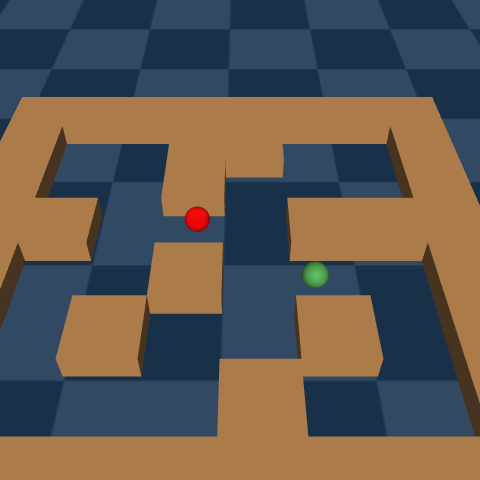
\includegraphics[width=0.25\textwidth]{experiments/figures/env.png}
    \caption{The pointmaze medium environment. The green ball is the actor and the red one is the goal.}
    \label{fig:envpic}
\end{figure}

The primary comparison conducted is shown in figure \ref{fig:smoothness_or_no}.
This comparison shows the effect of using the smoothness loss.
While the effect is mild, as more than half of the environments fail to reach even one goal in both cases, the smoothness constraint improves the result.
\begin{figure}
    \centering
    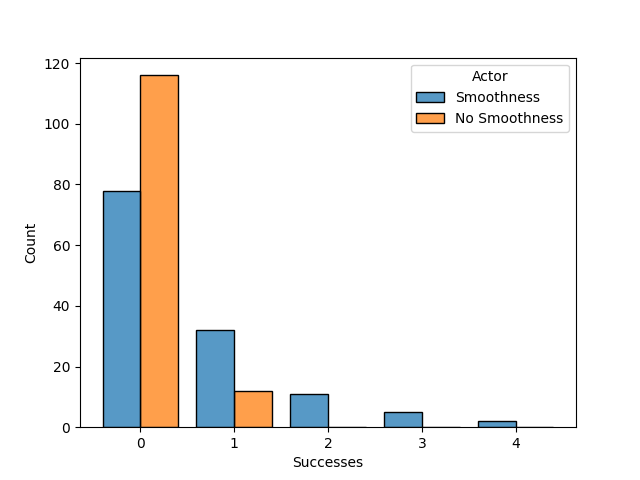
\includegraphics[width=0.45\textwidth]{experiments/figures/smoothness_or_no.png}
    \caption{
        This figure is a histogram which shows along the x-axis how many times a goal was reached in a trial.
        On the y-axis it shows the number of times that one of the trials achieved that number of goals (a new goal is set when one is reached).
        The orange bars show the results using a latent space with no smoothness constraint, and the blue bars show the results using a latent space with a smoothness constraint.
    }
    \label{fig:smoothness_or_no}
\end{figure}

The networks used were as follows
\begin{itemize}
    \item{State Encoder} Feed Forward Network, 3 hidden layers of size 1024, 512, 512
    \item{Action Encoder} Feed Forward Network, 3 hidden layers of size 512, 1024, 512
    \item{Transition Model} Transformer, 3 layers, 4 heads, 128 dimensional
    \item{State Decoder} Feed Forward Network, 3 hidden layers of size 1024, 512, 512
    \item{Action Decoder} Feed Forward Network, 3 hidden layers of size 512, 1024, 512
\end{itemize}

\section{Conclusion}

This result encouragess the hypothesis that a latent space designed for optimization can improve the results from trajectory optimization in latent spaces.
Investigation into deliberate ways to force latent world models to be amenable to optimization remains an exciting direction with these results showing that incorporating smoothness can significantly improve optimization outcomes.

\bibliographystyle{plain}
\bibliography{references}

\end{document}